
\documentclass[DIV=calc, paper=a4, fontsize=11pt, twocolumn, spanish]{scrartcl}	 % A4 paper and 11pt font size

\usepackage{lipsum} % Used for inserting dummy 'Lorem ipsum' text into the template
\usepackage[protrusion=true,expansion=true]{microtype} % Better typography
\usepackage{amsmath,amsfonts,amsthm} % Math packages
\usepackage[svgnames]{xcolor} % Enabling colors by their 'svgnames'
\usepackage[hang, small,labelfont=bf,up,textfont=it,up]{caption} % Custom captions under/above floats in tables or figures
\usepackage{booktabs} % Horizontal rules in tables
\usepackage{fix-cm}	 % Custom font sizes - used for the initial letter in the document
\usepackage[spanish]{babel}
\selectlanguage{spanish}
\usepackage[utf8]{inputenc}
\usepackage{graphicx}

\usepackage{sectsty} % Enables custom section titles
\allsectionsfont{\usefont{OT1}{phv}{b}{n}} % Change the font of all section commands

\usepackage{fancyhdr} % Needed to define custom headers/footers
\pagestyle{fancy} % Enables the custom headers/footers
\usepackage{lastpage} % Used to determine the number of pages in the document (for "Page X of Total")

% Headers - all currently empty
\lhead{}
\chead{}
\rhead{}

% Footers
\lfoot{}
\cfoot{}
\rfoot{\footnotesize Page \thepage\ of \pageref{LastPage}} % "Page 1 of 2"

\renewcommand{\headrulewidth}{0.0pt} % No header rule
\renewcommand{\footrulewidth}{0.4pt} % Thin footer rule

\usepackage{lettrine} % Package to accentuate the first letter of the text
\newcommand{\initial}[1]{ % Defines the command and style for the first letter
\lettrine[lines=3,lhang=0.3,nindent=0em]{
\color{DarkGoldenrod}
{\textsf{#1}}}{}}

%----------------------------------------------------------------------------------------
%	TITLE SECTION
%----------------------------------------------------------------------------------------

\usepackage{titling} % Allows custom title configuration

\newcommand{\HorRule}{\color{DarkGoldenrod} \rule{\linewidth}{1pt}} % Defines the gold horizontal rule around the title

\pretitle{\vspace{-30pt} \begin{flushleft} \HorRule \fontsize{35}{35} \usefont{OT1}{phv}{b}{n} \color{DarkRed} \selectfont} % Horizontal rule before the title

\title{Dilatación térmica de los sólidos} % Your article title

\posttitle{\par\end{flushleft}\vskip 0.2em} % Whitespace under the title

\preauthor{\begin{flushleft}\large \lineskip 0.5em \usefont{OT1}{phv}{b}{sl} \color{DarkRed}} % Author font configuration

\author{Sebastián Valencia, } % Your name

\postauthor{\footnotesize \usefont{OT1}{phv}{m}{sl} \color{Black} % Configuration for the institution name
Universidad de los Andes \\ 201111578

\par\end{flushleft}\HorRule} % Horizontal rule after the title



\date{} % Add a date here if you would like one to appear underneath the title block

%----------------------------------------------------------------------------------------

\begin{document}

\maketitle % Print the title

\thispagestyle{fancy} % Enabling the custom headers/footers for the first page 

%----------------------------------------------------------------------------------------
%	ABSTRACT
%----------------------------------------------------------------------------------------

% The first character should be within \initial{}
\initial{L}\textbf{os sólidos, están sujetos a transformaciones físicas y químicas al experimentar variaciones de temperatura. La dilatación térmica de los sólidos, es un fenómeno físico bien entendido y estudiado. Es necesario confirmar la intuición física haciendo uso de la experimentación. En la practica de laboratorio, se pretende hallar de manera experimental la constante de dilatación térmica de ciertos materiales, de esta forma, se confirma la intuición física y se  solidifica el entendimiento del método científico y la importancia de la experimentación}

%----------------------------------------------------------------------------------------
%	ARTICLE CONTENTS
%----------------------------------------------------------------------------------------

\section*{Objetivos}

\begin{enumerate}
\item Comprobar que la longitud de un objeto varia con la temperatura y medir el coeficiente de dilatación lineal del cobre y del aluminio.
\end{enumerate}


\section*{Marco teórico}

La mayoría de sustancias tienden a expandirse al aumentar su temperatura. Los líquidos lo hacen a nivel molecular, los sólidos de igual manera, pero sus implicaciones son más tangibles físicamente. Al aumentar la temperatura de una sustancia sólida, esta tiende a expandir su tamaño, es decir, aumentar sus dimensionales lineales, superficiales y volumétricas.

\subsection*{Expansión lineal}

Para el estudio teórico de la expansión térmica, se considera el caso más básico y completo de todos, pues explica de manera concisa las tres expresiones de la materia sólida (lineal, superficial y de volumen). El caso en cuestión, es la expansión térmica lineal. Para la deducción teórica, se tiene una vara de un material con longitud $L_o$, a una temperatura inicial $T_o$. Cuando la temperatura cambia a $T_o + \Delta T$, la longitud cambia a $L_o + \Delta L$. $\Delta L$, es proporcional al cambio en la temperatura. Por la ultima proposición, implica lo siguiente $\Delta L \sim L_o \Delta T$, lo que implica la presencia de cierta constante de proporcionalidad. 

$$\Delta L = \alpha L_o \Delta T$$

A partir de la anterior deducción, es posible probar que la longitud final de la vara es: $L_o + \Delta L = L_o + \alpha L_o \Delta T = L_o(1 + \alpha \Delta T)$. La constante de equivalencia, es llamada de expansión lineal del material.

\begin{figure}[htbp]
\centering
	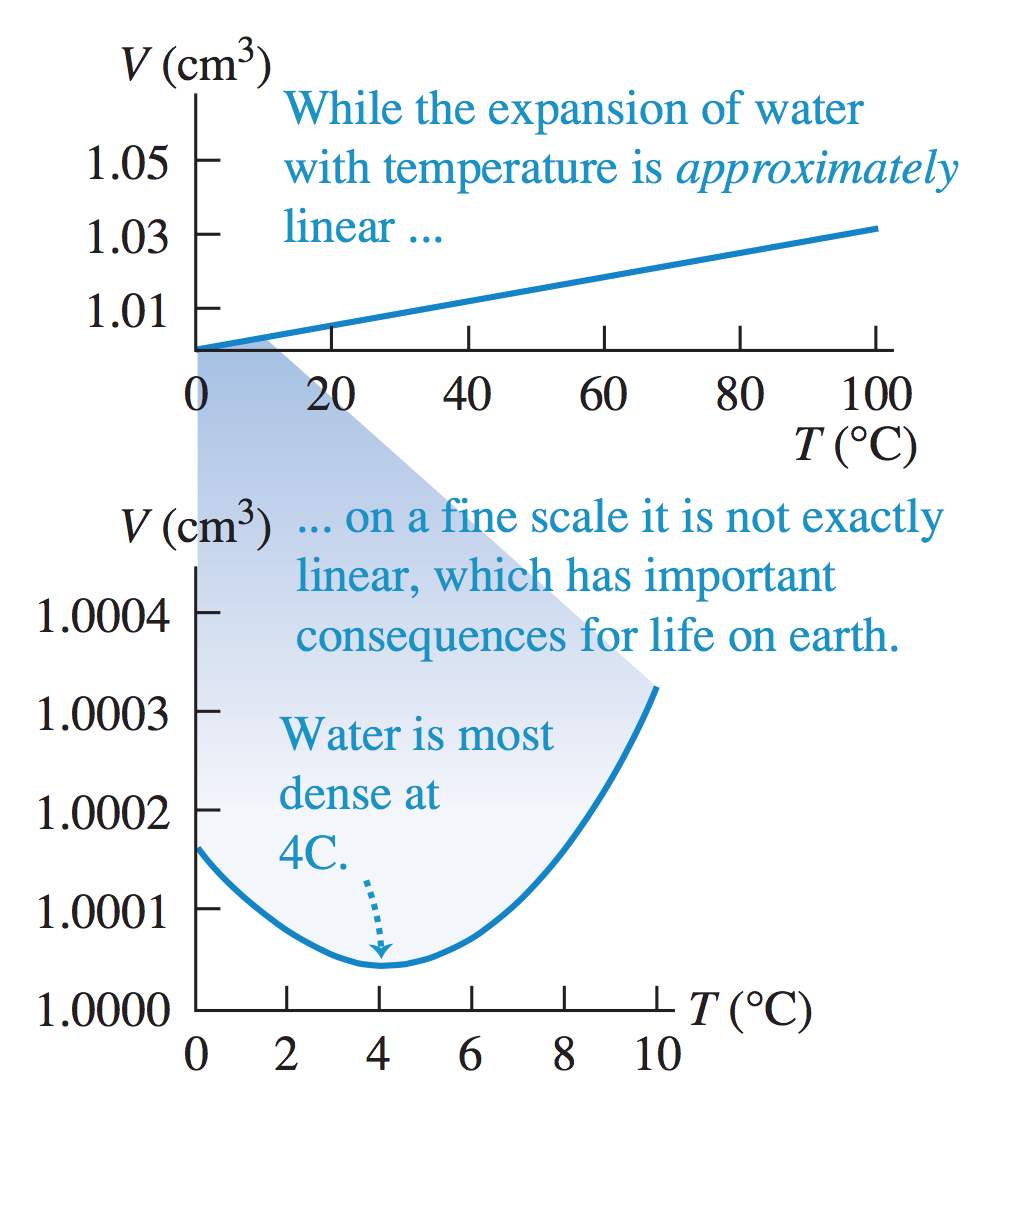
\includegraphics[scale=1]{data/img/figure01}
	\caption{Muestra la proporcianlidad que existe entre el cambio de temperatura, y el cambio de longitud. Imagen tomada de \cite{young2011sears}}
\end{figure}

\newpage

\section*{Procedimiento experimental}

La motivación para el procedimiento experimental en cuestión, es observar lo que ocurre al aumentar la temperatura de un tubo para distintos materiales. A través de esto, es pertinente registrar y verificar el aumento de longitud al aumentar la temperatura, además, se halla el coeficiente de expansión. Los materiales necesarios son:

\begin{itemize}
\item Tubos de aluminio y cobre.
\item Soporte para tubos
\item Manguera
\item Agua
\item Recipiente de agua
\item Estufa
\item Termómetro
\item Micrómetro
\item Soporte universal
\end{itemize}

\begin{figure}[htbp]
\centering
	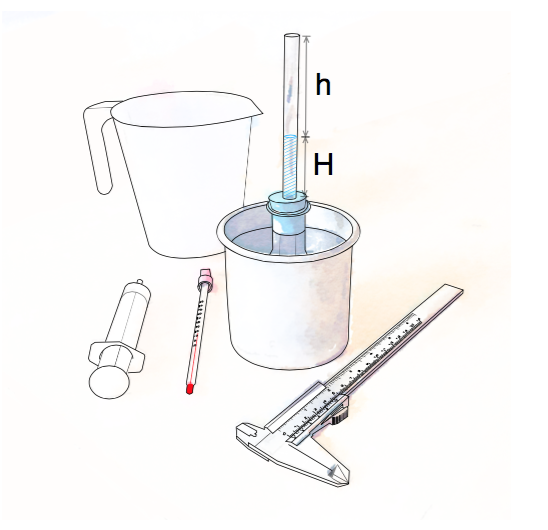
\includegraphics[scale=0.8]{data/img/figure02}
	\caption{Disposición de elementos para el desarrollo del laboratorio.}
\end{figure}

Se realiza el montaje asegurando la varilla entre las nueces dispuestas en los puntos $A$ y $B$. En el punto $B$, se aprisiona el micrómetro. Se registra la longitud $L_o$ entre los puntos $A$ y $B$, se registra la longitud $T_o$. La dirección del micrómetros, debe ser igual a la del tubo, la punta debe estar comprimida y en contacto con el tope sujeto al tubo.\\

Se calienta agua usando el recipiente y se conecta la manguera al recipiente. El micrómetro, se ubica para que la aguja coincida con 0, se asegura que el movimiento de la aguja del micrómetro indica la dilatación. Se prende la estufa y se deja el agua hervir, cuando la aguje deje de moverse, se registra el aumeto $\Delta L$, y $T_f$ en un extremo del tubo.

\section*{Análisis cualitativo}

\begin{enumerate}
\item Además de la medición directa que se hizo de $T_f$ , de que otra forma podría saberse la temperatura final sin usar un termómetro? Pensar, con que esta en contacto térmico la varilla?

Con la perdida gradual del volumen de agua y las leyes de transferencia de calor.

\item Al medir la temperatura en un extremo, qué idealización estamos haciendo?
\end{enumerate}

Que la difusión del calor se hace uniformemente en todo el material, sin pérdidas, ni malformaciones, además se presume que el material es puro.



%----------------------------------------------------------------------------------------
%	REFERENCE LIST
%----------------------------------------------------------------------------------------

\begin{thebibliography}{99} % Bibliography - this is intentionally simple in this template

  \bibitem{young2011sears} Sears and Zemansky.B. {\em Sears and Zemansky's University Physics / Tutorials in Introductory Physics / Tutorials in Introductory Physics Homework. 17:565--567}, Pearson Education.  2011.
 
\end{thebibliography}

%----------------------------------------------------------------------------------------

\end{document}